\documentclass[11pt]{article}

\linespread{1.0}

\newcommand{\bra}[1]{\left\langle #1 \right |}
\newcommand{\ket}[1]{\left | #1 \right\rangle}

\usepackage{mathtools}
\usepackage{floatrow}
\usepackage{bbold}
\usepackage{eurosym}
\usepackage{graphicx}
\usepackage{fullpage}
\usepackage{amsmath}
\usepackage{amsbsy}
\usepackage[all]{xy}
\usepackage[nottoc, notlof, notlot]{tocbibind}
\usepackage{makeidx}
\usepackage{multicol}
\usepackage{multirow}
\usepackage{float}
\usepackage{textcomp}
\usepackage[utf8]{inputenc}
\usepackage{bm}
\usepackage{appendix}
\usepackage{color}
\usepackage{listings}
\usepackage{slashed}
\usepackage{hyperref}
\usepackage{verbatim}
\usepackage{fancyhdr}
\usepackage{enumitem}
\usepackage[sans]{dsfont}
\usepackage{empheq}
\usepackage{feyn}
%\usepackage{noReferences}
\usepackage{booktabs}

\usepackage{array}
\newcolumntype{L}[1]{>{\raggedright\let\newline\\\arraybackslash\hspace{0pt}}m{#1}}
\newcolumntype{C}[1]{>{\centering\let\newline\\\arraybackslash\hspace{0pt}}m{#1}}
\newcolumntype{R}[1]{>{\raggedleft\let\newline\\\arraybackslash\hspace{0pt}}m{#1}}

\usepackage[headsep=0.8cm,headheight=0cm]{geometry}

\setlength{\oddsidemargin}{0.25in}
\setlength{\hoffset}{0.2in}
\setlength{\textwidth}{5.8in}
\setlength{\topmargin}{0.2in}
\setlength{\voffset}{-0.5in}
\setlength{\textheight}{8.8in}

\pagestyle{fancy}

\fancyhf{}
\lhead{The Bubble Problem}
%\rhead{Dr. Valentin Hirschi}
\rfoot{\thepage}


\definecolor{colKeys}{rgb}{0,0,1}
\definecolor{colIdentifier}{rgb}{0,0,0}
\definecolor{colComments}{rgb}{0,0.5,1}
\definecolor{colString}{rgb}{0.6,0.1,0.1}

\lstset{%configuration de listings
float=hbp,%
basicstyle=\ttfamily\small, %
identifierstyle=\color{colIdentifier}, %
keywordstyle=\color{colKeys}, %
stringstyle=\color{colString}, %
commentstyle=\color{colComments}, %
columns=flexible, %
tabsize=2, %
frame=trBL, %
frameround=tttt, %
extendedchars=true, %
showspaces=false, %
showstringspaces=false, %
numbers=left, %
numberstyle=\tiny, %
breaklines=true, %
breakautoindent=true, %
captionpos=b,%
}

\date{\today}

\makeatletter
\renewcommand\theequation{\thesection.\arabic{equation}}
\@addtoreset{equation}{section}
\makeatother

\makeatletter
\renewcommand{\thefigure}{\ifnum \c@section>\z@ \thesection.\fi
 \@arabic\c@figure}
\@addtoreset{figure}{section}
\makeatother

\newcommand\captionof[1]{\def\@captype{#1}\caption}
\newcommand\MadFKS{{\sc\small MadFKS}}
\newcommand\CutTools{{\sc\small CutTools}}
\newcommand\OneLOop{{\sc\small OneLOop}}
\newcommand\MadLoop{{\sc\small MadLoop}}
\newcommand\PROSPINO{{\sc\small PROSPINO}}
\newcommand\ML{{\sc\small ML}}
\newcommand\ResearchPlanTitle{{Automation of beyond-NLO accurate predictions for particle colliders}}
\newcommand\TitleScaleUp{1.02}
\newcommand\MadEvent{{\sc\small MadEvent}}
\newcommand\MadGraph{{\sc\small MadGraph5}}
\newcommand\MGaMC{{\sc\small MadGraph5\_aMC@NLO}}
\newcommand\Mathematica{{\sc\small Mathematica}}
\newcommand\FeynRules{{\sc\small FeynRules}}
\newcommand\MGF{{\sc\small MG5}}
\newcommand\Vincia{{\sc\small Vincia}}
\newcommand\BlackHat{{\sc\small BlackHat}}
\newcommand\MCatNLO{{\sc\small MC@NLO}}
\newcommand\aMCatNLO{{\sc\small aMC@NLO}}
\newcommand\HELAS{{\sc\small HELAS}}
\newcommand\Alpgen{{\sc\small Alpgen}}
\newcommand\Sherpa{{\sc\small Sherpa}}
\newcommand\Herwig{{\sc\small Herwig}}
\newcommand\Pythia{{\sc\small Pythia}}
\newcommand\COLLIER{{\sc\small COLLIER}}
\newcommand\PJFrypp{{\sc\small PJFry++}}
\newcommand\MCFM{{\sc\small MCFM}}
\newcommand\qpart{q^\star}
\newcommand\qbpart{\bar{q}^\star}
\newcommand\sss{\scriptscriptstyle}
\newcommand\as{\alpha_{\sss S}}
\newcommand\gs{g_{\sss S}}
\newcommand\aW{\alpha_{\sss W}}
\newcommand\mtop{m_{top}}
\newcommand\mQ{m_Q}
\newcommand\muF{\mu_{\sss F}}
\newcommand\muR{\mu_{\sss R}}

\newcommand\textbox[1]{%
  \parbox{.333\textwidth}{#1}%
}
% A small hack to have coloured comment in the tex file  without using colour package
% It's ok since there will be no comments left for the final version
\chardef\MyArticleWithColor=\pdfcolorstackinit page direct{0 g}
\def\cmtVH#1{\emph{\pdfcolorstack\MyArticleWithColor push {1 0 0 rgb} V.H. : #1 \pdfcolorstack\MyArticleWithColor pop}}

\newcommand{\pbox}[4]{
\psshadowbox[#3]{
\begin{minipage}[t][#2][t]{#1}
#4
\end{minipage}
}}

%\setlist[itemize]{leftmargin=0cm, topmargin=0.5cm, bottommargin=0.5cm}

\newcommand{\note}[1]
   {\footnote{$\,$#1}}

%\renewcommand{\thesection}{\thesection.\alph{section}}
\renewcommand{\thesection}{\alph{section}}

\begin{document}

%\input{Title}
%\setcounter{page}{1}
\pagenumbering{gobble}
\phantom{.}\vspace{-0.5cm}
\section{The bubble problem: dispersion relation at the rescue}

The squared LTD program faces the difficulty of addressing 1-Particle-Irreducible (1PI) self-energy energy diagrams as the one below in Fig.~\ref{TheBubbleProblem} when the Cutkosky cut goes to the left and right of it.

\begin{figure}[ht!]
\begin{center}
\begin{minipage}{0.65\linewidth}
\centering
{\caption{\label{TheBubbleProblem} Illustrative example of the bubble problem in the squared LTD programme.}}
{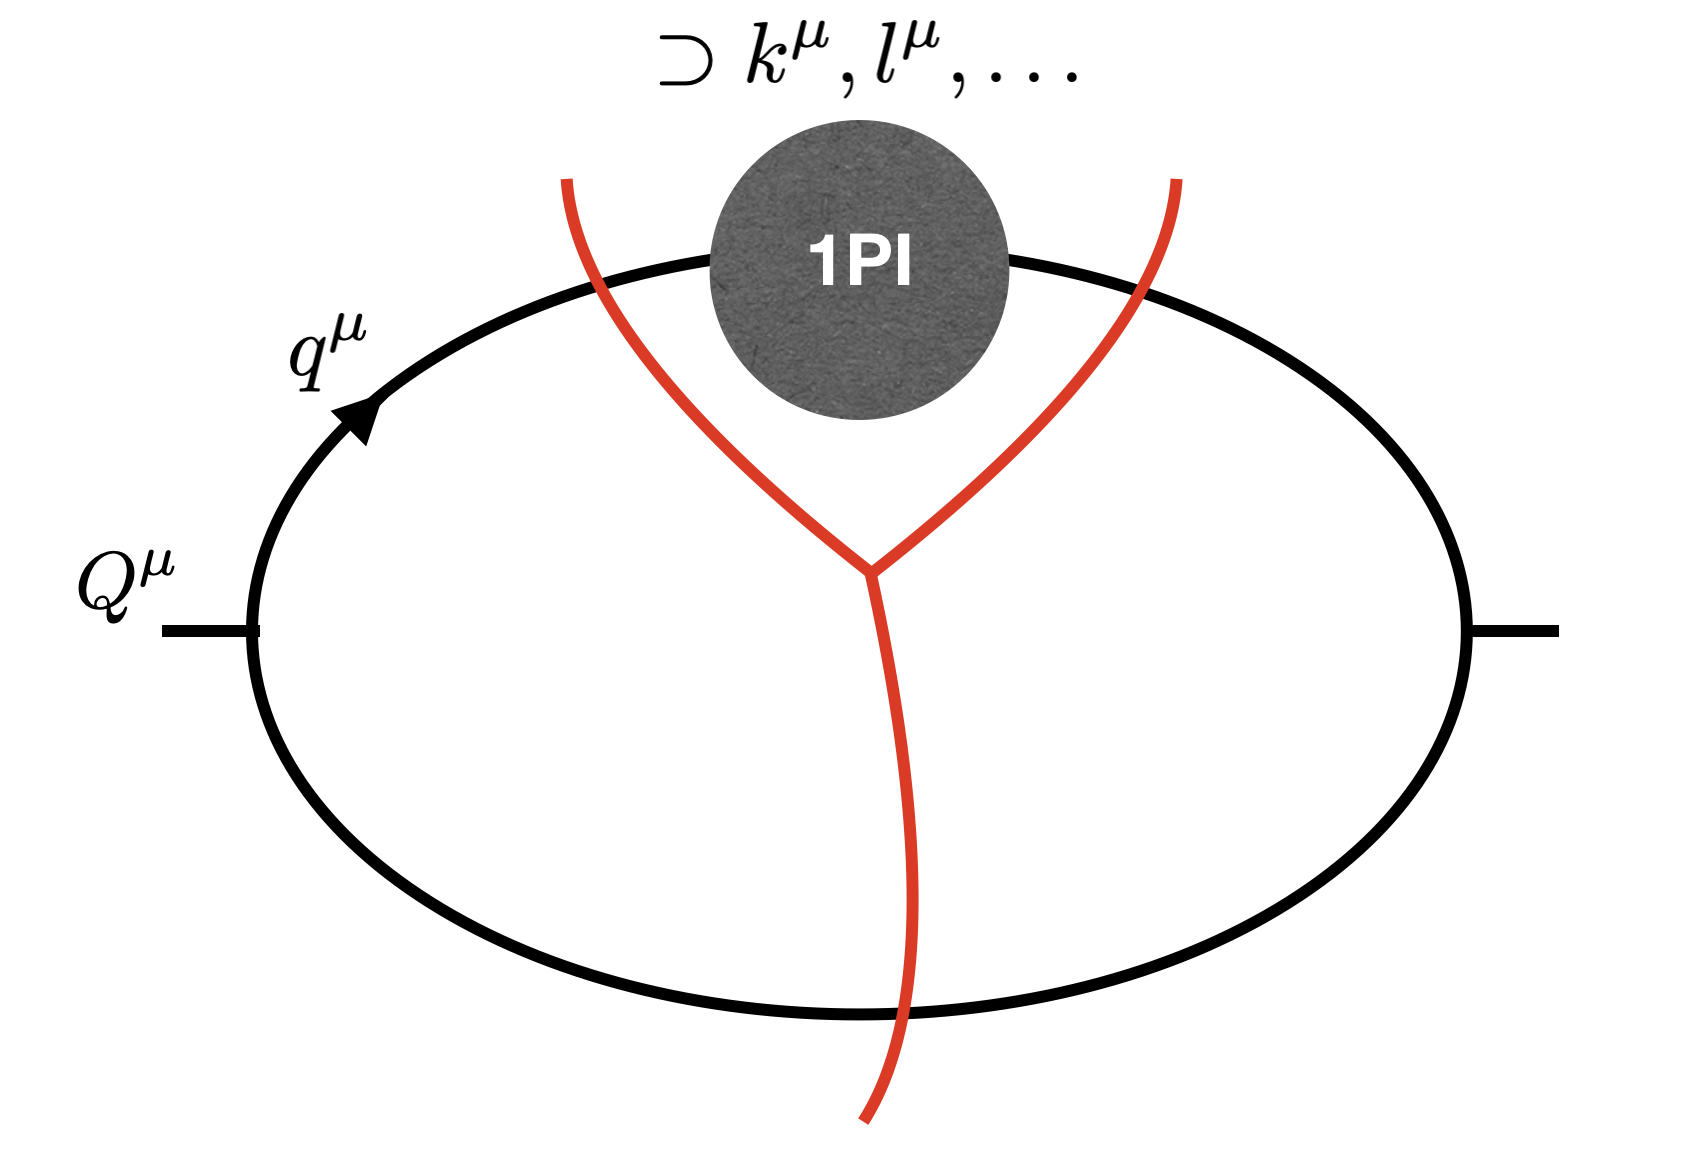
\includegraphics[width=0.65\linewidth]{the_bubble_problem.png}}
\end{minipage}\hfill
\end{center}
\end{figure}

\noindent We will denote the 1PI bubble $\Sigma_{ij}(q^0, \vec{q})$ where $i,j$ are indices in the Lorentz representation of the particle dressed subject to this self-energy. More precisely, we will define $\Sigma_{ij}$ as:

\begin{equation}
\Sigma_{ij}(q^0, \vec{q}) =\int \prod_{i=1}^{N} \left(\frac{d^4 k_i}{(2\pi)^4}\right)  \frac{ \mathcal{N} \left(  q^0, \vec{q} ; \{ (k_i^0, \vec{k_i}) \} \right) } {\prod_{j=1}^{N_d} D_j}
\end{equation}

The problem we are facing is in making the quantity $\frac{\Sigma_{ij}(q^0, \vec{q})}{q^2}$ \emph{locally} finite and reproducing the correct physical results, both in terms of cancelling the IR divergences of the real-emission Cutkosky cut of the supergraph of Fig.~\ref{TheBubbleProblem} and also in terms of reproducing the results from traditional computations done with a dimensional regulator in the on-shell renormalisation scheme.

To this end, we will take advantage of the dispersion relation for $\Sigma_{ij}$ which takes advantage of our knowledge that such two point functions only feature branch cuts along the real axis. We can then consider the following two integration contours of Fig.~\ref{IntegrationContours}.

\begin{figure}[ht!]
\begin{center}
\begin{minipage}{0.65\linewidth}
\centering
{\caption{\label{IntegrationContours} Integration contours considered for deriving the dispersion relation.}}
{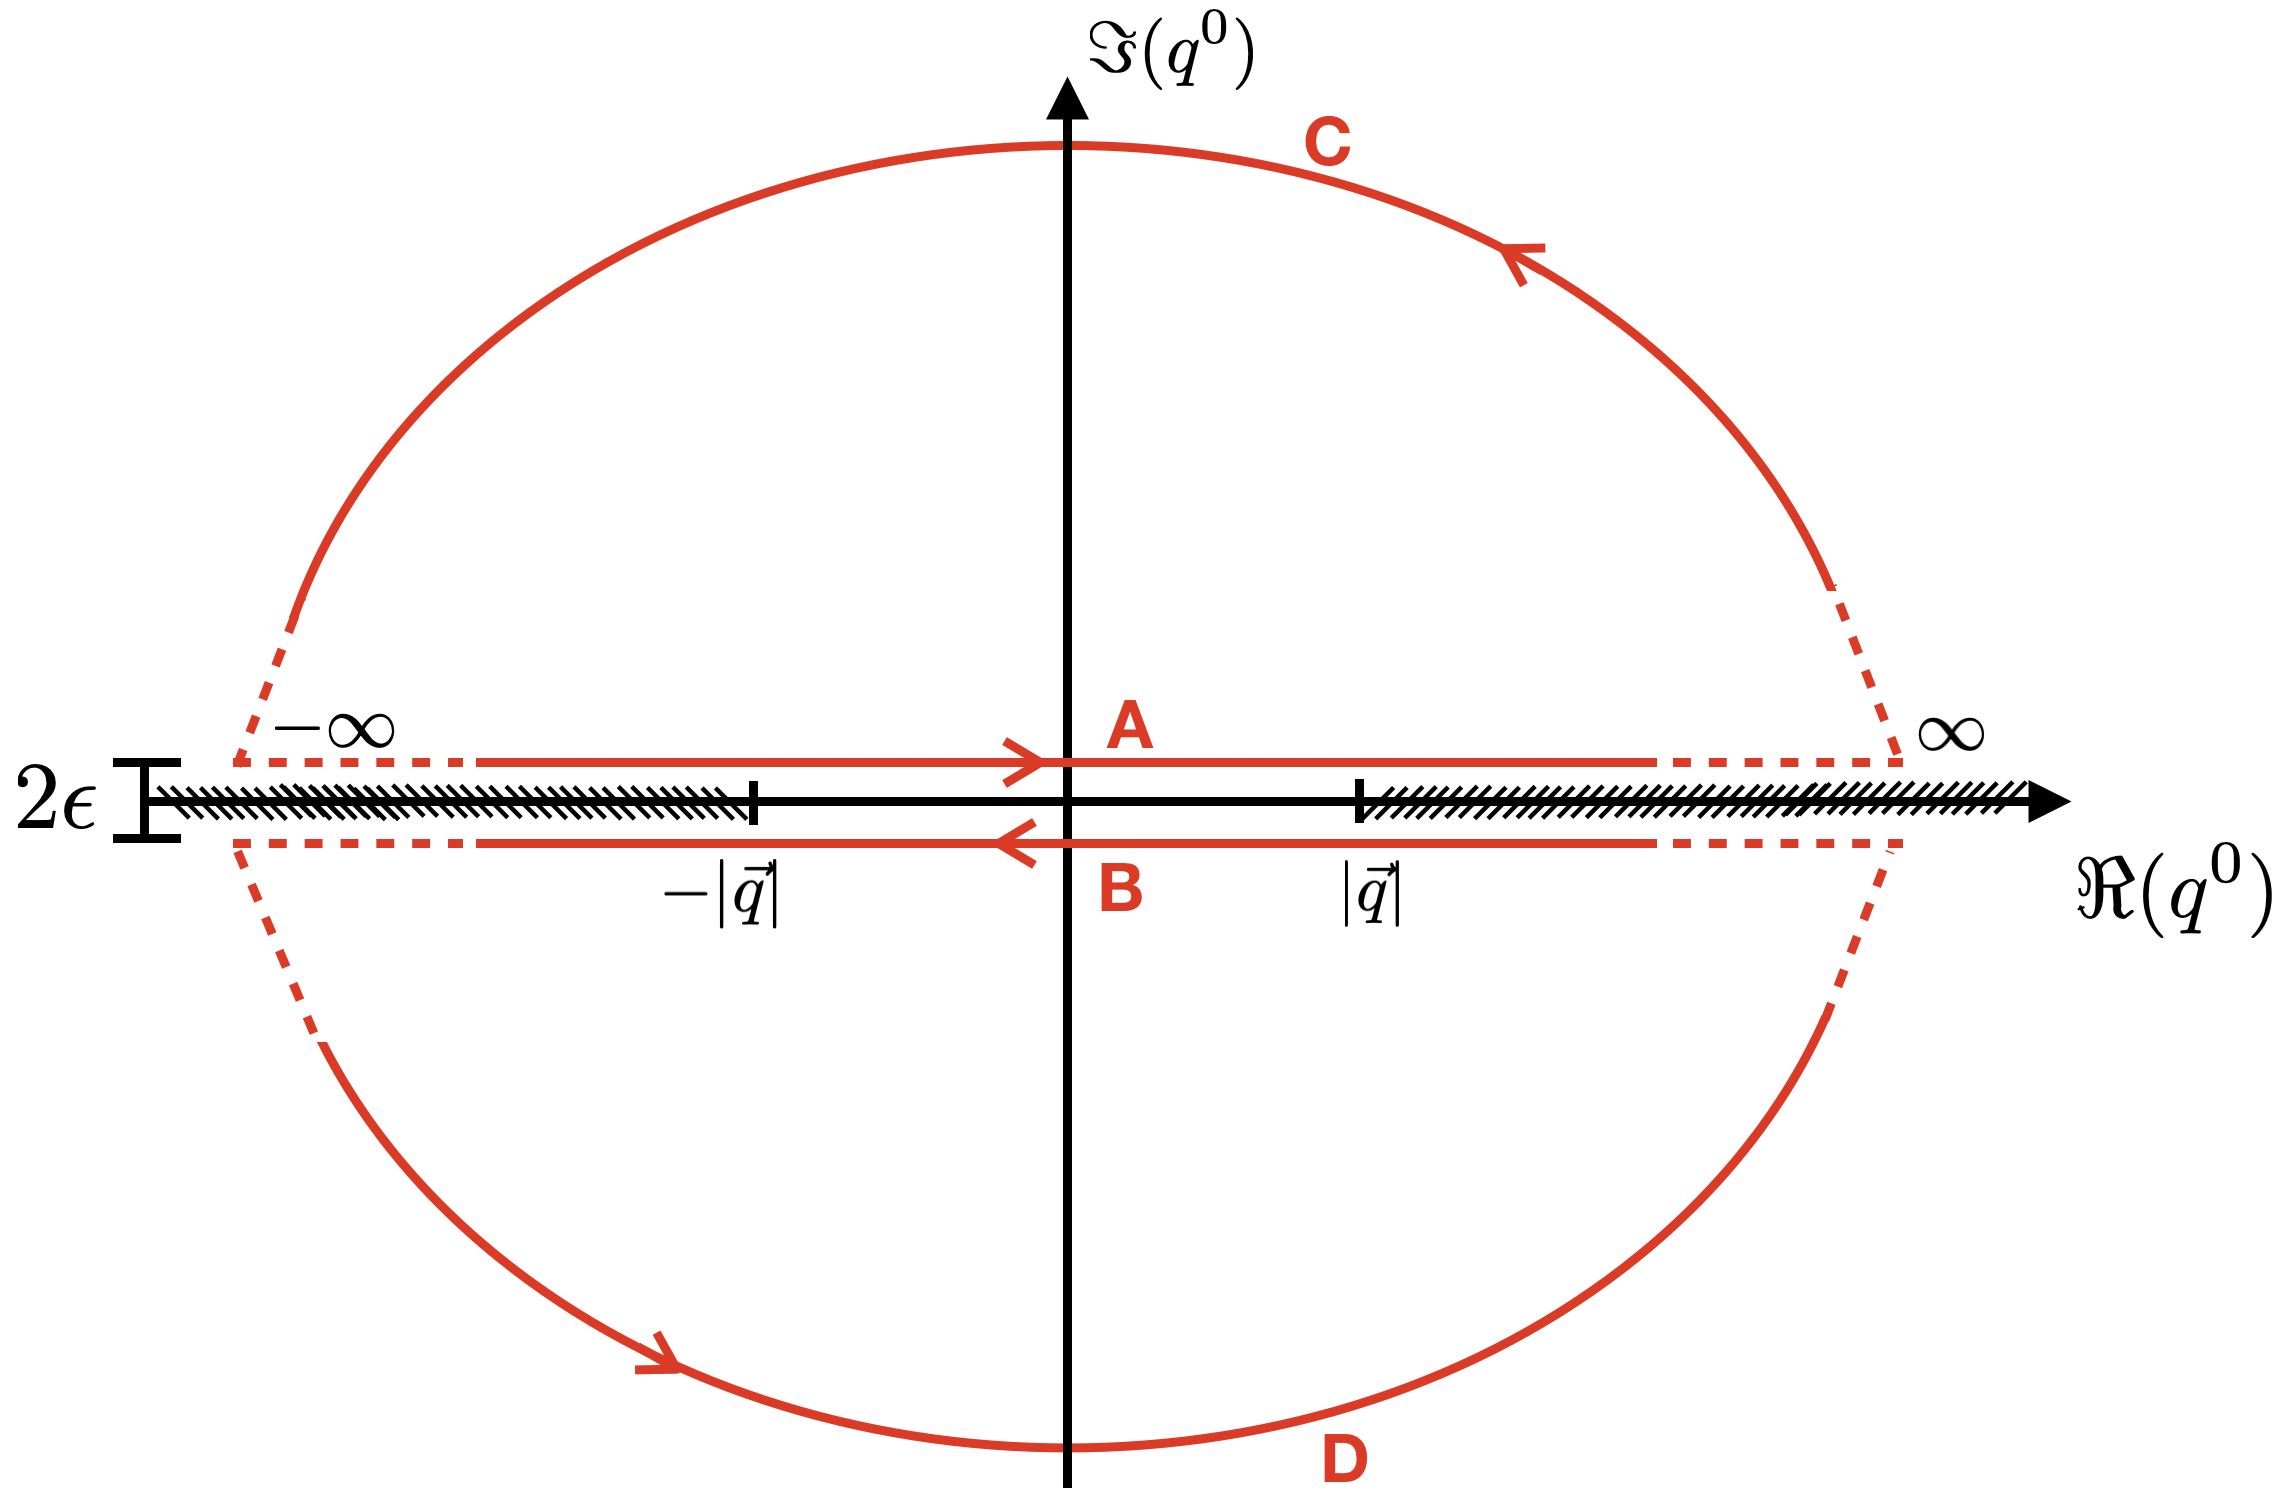
\includegraphics[width=0.65\linewidth]{integration_contour.png}}
\end{minipage}\hfill
\end{center}
\end{figure}

Using Cauchy theorem, we can write this simple identity for $\Sigma_{ij}(q^0, \vec{q})$, valid for any value of $q^0$ \emph{not} on a branch-cut of the real-axis, indicated as a hashed area in Fig.~\ref{IntegrationContours}:
\begin{eqnarray}
\Sigma_{ij}(q^0, \vec{q}) &=& \lim_{\epsilon \rightarrow 0^+}\frac{1}{2\pi i} \left[ 
\underbrace{ \int_{-\infty}^\infty d z \frac{ \Sigma_{ij}(z+i\epsilon, \vec{q}) }{z-q^0+i\epsilon} }_{\textrm{segment A}} +
\underbrace{ \int_{\infty}^{-\infty} d z \frac{ \Sigma_{ij}(z-i\epsilon, \vec{q}) }{z-q^0-i\epsilon} }_{\textrm{segment B}}
\right ] \nonumber \\
&=& 
\frac{1}{2\pi i}  \lim_{\epsilon \rightarrow 0^+} \int_{-\infty}^\infty d z \frac{ \Sigma_{ij}(z+i\epsilon, \vec{q}) -  \Sigma_{ij}(z-i\epsilon, \vec{q})  }{z-q^0} \nonumber \\
&=&
\frac{1}{2\pi i} \int_{-\infty}^\infty d z \frac{ \textrm{disc} \left[ \Sigma_{ij}(z, \vec{q}) \right] }{z-q^0},\label{DispertionRelation}
\end{eqnarray}
where we neglected the $\pm i \epsilon$ in the denominators of the second line because we assume that $\Sigma_{ij}$ is analytic everywhere except on the branch cuts of the real axis which our contour never crosses. We also used the assumption that $\lim_{|z| \rightarrow \infty} \Sigma_{ij}(z, \vec{q}) = 0$, allowing us to neglect the segments C and D of the contour at infinity.
As shown by the Cutkosky cuts of Fig.~\ref{TheBubbleProblem}, we are eventually interested in evaluating this contribution at $q^0=\sqrt{|\vec{q}|^2+m^2}$. It therefore proves useful to consider the difference of $\Sigma_{ij}$ evaluated at a generic $q^0$ and at $\sqrt{|\vec{q}|^2+m^2}$, both time re-expressing the result using Eq.~\ref{DispertionRelation}:
\begin{eqnarray}
&&\Sigma_{ij}(q^0, \vec{q}) - \Sigma_{ij}(\sqrt{|\vec{q}|^2+m^2}, \vec{q}) = 
\frac{1}{2\pi i} \int_{-\infty}^\infty d z \frac{ \textrm{disc} \left[ \Sigma_{ij}(z, \vec{q}) \right] }{z-q^0}
-
\frac{1}{2\pi i} \int_{-\infty}^\infty d z \frac{ \textrm{disc} \left[ \Sigma_{ij}(z, \vec{q}) \right] }{z-\sqrt{|\vec{q}|^2-m^2}} \nonumber \\
&&\Sigma_{ij}(q^0, \vec{q}) = \Sigma_{ij}(\sqrt{|\vec{q}|^2+m^2}, \vec{q}) +
\frac{1}{2\pi i} \int_{-\infty}^\infty d z \frac{ 
\textrm{disc} \left[ \Sigma_{ij}(z, \vec{q}) \right] \left( (z-\sqrt{|\vec{q}|^2-m^2}) -  (z-q^0) \right)
}{( z-q^0) (z-\sqrt{|\vec{q}|^2-m^2}) } \nonumber \\
&&\Sigma_{ij}(q^0, \vec{q}) = \Sigma_{ij}(\sqrt{|\vec{q}|^2+m^2}, \vec{q}) +
\frac{q^0 -\sqrt{|\vec{q}|^2-m^2} }{2\pi i} \int_{-\infty}^\infty d z \frac{ 
\textrm{disc} \left[ \Sigma_{ij}(z, \vec{q}) \right]
}{( z-q^0) (z-\sqrt{|\vec{q}|^2-m^2}) }\label{SubtractionProcedure}
\end{eqnarray}
Our goal is to use squared LTD to reproduce the computation of a \emph{renormalised} (in the On-Shell (OS) scheme for external wavefunctions) scattering cross-section, for which the super graph of Fig.~\ref{TheBubbleProblem} is supposed to also capture the \emph{renormalised} self-energy insertion, that is $\Sigma_{ij}^{(OS)}(q^0, \vec{q})=\Sigma_{ij}(q^0, \vec{q})+\delta Z^{(OS)}_{ij}$, with the wavefunction counterterm $\delta Z^{(OS)}_{ij}$ defined such that $\Sigma_{ij}^{(OS)}(\sqrt{|\vec{q}|^2+m^2}, \vec{q})=0$, so that $\delta Z^{(OS)}_{ij}=-\Sigma_{ij}(\sqrt{|\vec{q}|^2+m^2}, \vec{q})$.\\
We thus get:
\begin{eqnarray}
\Sigma_{ij}^{(OS)}(q^0, \vec{q}) &=& \Sigma_{ij}(\sqrt{|\vec{q}|^2+m^2}, \vec{q}) + \delta Z^{(OS)}_{ij} +
\frac{q^0 -\sqrt{|\vec{q}|^2-m^2} }{2\pi i} \int_{-\infty}^\infty d z \frac{ 
\textrm{disc} \left[ \Sigma_{ij}(z, \vec{q}) \right]
}{( z-q^0) (z-\sqrt{|\vec{q}|^2-m^2}) } \nonumber \\
&=& \frac{q^0 -\sqrt{|\vec{q}|^2-m^2} }{2\pi i} \int_{-\infty}^\infty d z \frac{ 
\textrm{disc} \left[ \Sigma_{ij}(z, \vec{q}) \right]
}{( z-q^0) (z-\sqrt{|\vec{q}|^2-m^2}) }
\end{eqnarray}
Note that this renormalisation argument with the introduction of the complete OS wavefunction renormalisation counterterm is possibly more complicated beyond one-loop since we will be considering only one multi-loop bubble topology at a time and the counterterms of course always refer to the complete sum of all 1PI contributions.
But it may still be that it trivially generalises.
We can now write down our particular ratio of interest, this time regularised:
\begin{equation}
\overline{\Sigma}_{ij}^{(OS)}(q^0, \vec{q}) \vcentcolon= \frac{\Sigma_{ij}^{(OS)}(q^0, \vec{q})}{(q^0)^2-|\vec{q}|^2-m^2} = \frac{ 1 }{2\pi i} \frac{1}{q^0 + \sqrt{|\vec{q}|^2-m^2 }} \int_{-\infty}^\infty d z \frac{ 
\textrm{disc} \left[ \Sigma_{ij}(z, \vec{q}) \right]
}{( z-q^0) (z-\sqrt{|\vec{q}|^2-m^2}) },
\end{equation}
which can now safely be evaluated at $q^0 = \sqrt{|\vec{q}|^2-m^2 }$ :
\begin{equation}
\overline{\Sigma}_{ij}^{(OS)}(\sqrt{|\vec{q}|^2-m^2 }, \vec{q}) = \frac{ 1 }{2\pi i} \frac{1}{2\sqrt{|\vec{q}|^2-m^2 }} \int_{-\infty}^\infty d z \frac{ 
\textrm{disc} \left[ \Sigma_{ij}(z, \vec{q}) \right]
}{\left( z-\sqrt{|\vec{q}|^2-m^2 }\right)^2 }.
\label{FinalDiscExpressionBubbleProblem}
\end{equation}
In order to expose the exact same denominator structure as in the original super graph of Fig.~\ref{TheBubbleProblem}, we can rewrite the expression above as:
\begin{eqnarray}
&&\overline{\Sigma}_{ij}^{(OS)}(\sqrt{|\vec{q}|^2-m^2 }, \vec{q}) = 
\frac{ 1 }{2\pi i} \frac{1}{2\sqrt{|\vec{q}|^2-m^2 }} \int_{-\infty}^\infty d z \frac{ 
\textrm{disc} \left[ \Sigma_{ij}(z, \vec{q}) \right]
}{\left( z-\sqrt{|\vec{q}|^2-m^2 }\right)^2 } \frac{\left( z + \sqrt{|\vec{q}|^2-m^2 }\right)^2}{\left( z + \sqrt{|\vec{q}|^2-m^2 }\right)^2} \nonumber \\
&=& 
\frac{ 1 }{2\pi i} \frac{1}{2\sqrt{|\vec{q}|^2-m^2 }} \int_{-\infty}^\infty d z \frac{ 
\textrm{disc} \left[ \Sigma_{ij}(z, \vec{q}) \right] \left( z + \sqrt{|\vec{q}|^2-m^2 }\right)^2
}{( z^2 - |\vec{q}|^2-m^2)^2 },\label{FinalExpressionBubbleProblemWithMatchingProps}
\end{eqnarray}
thus making the contribution identical in structure to that of the original problematic super graph, except that this time the energy $q^0$ is no longer set to the solution $\sqrt{|\vec{q}|^2-m^2}$ from the on-shell constraint but instead set to $z$ and integrated over.

We will now work on giving an alternative and more explicit expression for the discontinuity of $\Sigma_{ij}(z, \vec{q})$ by taking advantage of the fact that all 1 PI self-energy satisfy (at any order in perturbation theory and also for massive internal lines (?) ) the reality condition known as the \emph{Schwartz reflection principle}, namely:
\begin{equation}
\Sigma_{ij}(z^*, \vec{q})=\Sigma_{ij}(z, \vec{q})^*
\end{equation}
which allows us to rewrite the discontinuity as:
\begin{eqnarray}
\textrm{disc} \left[ \Sigma_{ij}(z, \vec{q}) \right] &=& \lim_{\epsilon->0^+} \left( \Sigma_{ij}(z+i\epsilon, \vec{q}) - \Sigma_{ij}(z-i\epsilon, \vec{q}) \right ) \nonumber \\
&=&  \lim_{\epsilon \rightarrow 0^+} \left( \Sigma_{ij}(z+i\epsilon, \vec{q}) - \Sigma_{ij}(z+i\epsilon, \vec{q})^* \right )\nonumber \\
&=&  2 i \lim_{\epsilon \rightarrow 0^+}  \Im{ \left[ \Sigma_{ij}(z+i\epsilon, \vec{q}) \right] } \nonumber \\
&=&  i \sum_{\textrm{C}_i\in\{\textrm{Cutkosky cuts}\}} \textrm{C}_i\left[ \Sigma_{ij}(z, \vec{q})\right ].\label{DiscIntoCutkosky}
\end{eqnarray}
\cmtVH{TODO: WARNING: LIKELY WRONG!\ Above applies only if z is positive!\ We must therefore split the integration $\int_{-\infty}^{+\infty}$ into two pieces $\int_{0}^{+\infty}$ like Soper did in order to apply Cutkosky.}
Where the last equality holds from a stronger version of the optical theorem that relates the imaginary part of the 1PI to the list of all Cutkosky cuts of the super graph.  
Actually, the detour of re-expressing the discontinuity in terms of the imaginary part through the Schwartz reflection principle is probably a distraction and even wrong since we are only considering one particular bubble at a time and not all of them which is what the only case strictly speaking addressed by the optical theorem.
I only included it here as I think it may be useful to keep in mind.
Instead, I believe that in practice all what we really need to invoke is just the Cutkosky rule that expresses the discontinuity of loop integrals, as written in Eq. (55) of ref.~\cite{Zwicky:2016lka}.

One nice observation of Eq.~\ref{DiscIntoCutkosky} is that this rewriting of the "on-shell Bubble" through Cutkosky shows very clearly how the IR cancellation with the corresponding real-emission cut super-graph occurs: all the on-shell conditions between the "virtual" and "real" bubble are now lined up and it is clear from Eq.~\ref{FinalExpressionBubbleProblemWithMatchingProps} how the integrands of these two contributions become identical when $q^2=0$!

Finally, notice that the sum over Cutkosky cuts in Eq.~\ref{DiscIntoCutkosky} can also be interpreted as a sum over Dirac delta's imposing that $z$ to sit on each of the \emph{existing} E-surfaces of the (multi-)loop bubble.
The non-existing E-surfaces indeed give no imaginary part, and also have no real-emission counterpart as they would not have phase-space support.
These cuts do not necessarily set the energy of all loop momenta, for example in the case of a one-loop type of E-surface of a two-loop bubble. There again, such a case has an analogous real-emission contribution in the form of a one-loop final-state splitting.

Our final expression of the \emph{regularised} 1PI self-energy therefore reads:
\begin{equation}
\overline{\Sigma}_{ij}^{(OS)}(\sqrt{|\vec{q}|^2-m^2 }, \vec{q}) = \frac{ 1 }{2\pi} \frac{1}{2\sqrt{|\vec{q}|^2-m^2 }} 
\int_{-\infty}^\infty dz \frac{ 
\sum_{C_i \in \mathcal{C}_\Sigma} C_i\left[ \Sigma_{ij}(z, \vec{q})\right] \left( z + \sqrt{|\vec{q}|^2-m^2 }\right)^2
}{( z^2 - |\vec{q}|^2-m^2)^2 } \;
\label{FinalResult},
\end{equation}
\cmtVH{PROBABLY WRONG RESULT, we need to split the integration range $\int_{-\infty}^{+\infty}$ into two pieces $\int_{0}^{+\infty}$ like Soper did and compute differently the discontinuity for positive and negative energies!\ Eq.~\ref{FinalExpressionBubbleProblemWithMatchingProps} should be correct though.}
where $\mathcal{C}_\Sigma$ is the set of \emph{all} Cutkosky cut operators $C_i$ of the 1PI self-energy graph considered.
The cutkosky cut operators $C_i$ are of the form $C_i \sim (-2\pi i)^{|\textrm{cuts}_i|} \prod_{j\in \textrm{cuts}_i} q_j^2(z) \delta^+\left(q_j^2(z)\right)$.\\
Our finding suggests that \emph{all} contributions from \emph{regularised} and \emph{renormalised} 1PI (multi-)loop bubbles have a phase-space support identical to that of another existing real-emission Cutkosky cut of the same super graph. It therefore seems that structurally, a sound strategy for implementing it in {\sc\small RUST} is to completely ignore the self-energy bubbles contributions and instead complement all real-emission Cutkosky cuts of the same super graph with the one corresponding contribution appearing in the sum on the r.h.s of Eq.~\ref{FinalResult}. This also works well with the fact that if the above result is correct, it suggests that the LTD procedure (i.e. integration over the energy of the \emph{remaining} loops) should start *only* after the Cutkosky operator $C_i$ has been applied.
One main difference w.r.t our previous understanding of Friday, February 21$^\textrm{st}$ is thus that in the one-loop case of Soper for example, the loop energy $k^0$ is \emph{not} set from the LTD procedure but instead from the application of the $Cutkosky$ cut.
If the understanding above is correct, the LTD procedure would kick in \emph{only} if there are still loops left after the application fo the Cutkosky cut $C_i$.

\vspace{4cm}
\noindent ERRATUM: In order to be able to correctly apply the Cutkosky rule, we must start from Eq.~\ref{FinalExpressionBubbleProblemWithMatchingProps} and split the integration range $\int_{-\infty}^{+\infty}$ into two pieces $\int_{0}^{+\infty}$ like Soper did.
\begin{eqnarray}
\label{MasterBubbleFormula}
&&\overline{\Sigma}_{ij}^{(OS)}(\sqrt{|\vec{q}|^2-m^2 }, \vec{q}) = 
\frac{ 1 }{2\pi i} \frac{1}{2\sqrt{|\vec{q}|^2-m^2 }} \int_{-\infty}^\infty d z \frac{ 
\textrm{disc} \left[ \Sigma_{ij}(z, \vec{q}) \right] \left( z + \sqrt{|\vec{q}|^2-m^2 }\right)^2
}{( z^2 - |\vec{q}|^2-m^2)^2 } \nonumber\\
&=& 
\frac{ 1 }{2\pi i} \frac{1}{2\sqrt{|\vec{q}|^2-m^2 }} \int_{0}^\infty d z \frac{ 
\textrm{disc} \left[ \Sigma_{ij}(z, \vec{q}) \right] \left( z + \sqrt{|\vec{q}|^2-m^2 }\right)^2
+ \textrm{disc} \left[ \Sigma_{ij}(-z, \vec{q}) \right] \left( -z + \sqrt{|\vec{q}|^2-m^2 }\right)^2
}{( z^2 - |\vec{q}|^2-m^2)^2 }\nonumber \\
\label{FinalExpressionBubbleProblemWithSplitRange}
\end{eqnarray}
If we now invoke the \emph{Schwartz reflection principle}:
\begin{equation}
\Sigma[z^*,\vec{q}]=\Sigma[z,\vec{q}]^* 
\;\;\;\rightarrow\;\;\; 
\textrm{disc} \left[ \Sigma_{ij}(z, \vec{q}) \right]=2i \lim_{\epsilon\rightarrow 0^+}\Im[\Sigma_{ij}(z, \vec{q})]
\end{equation}
and the \emph{crossing symmetry} of the 1PI self-energy (which we note to be in general \emph{not} applicable):
\begin{equation}
\lim_{\epsilon\rightarrow 0^+} \Sigma[-z\pm i \epsilon,\vec{q}]=\lim_{\epsilon\rightarrow 0^+} \Sigma[z\pm i\epsilon,\vec{q}]^*
\;\;\;\rightarrow\;\;\; 
\textrm{disc} \left[ \Sigma_{ij}(-z, \vec{q}) \right] = -\textrm{disc} \left[ \Sigma_{ij}(z, \vec{q}) \right],
\end{equation}
we can then simplify Eq.~\ref{FinalExpressionBubbleProblemWithSplitRange} as follows:
\begin{eqnarray}
&&\overline{\Sigma}_{ij}^{(OS)}(\sqrt{|\vec{q}|^2-m^2 }, \vec{q})= \nonumber\\ 
&&\frac{ 1 }{2\pi i} \frac{1}{2\sqrt{|\vec{q}|^2-m^2 }} \int_{0}^\infty d z \frac{ 
\textrm{disc} \left[ \Sigma_{ij}(z, \vec{q}) \right] 
\left( 
\left( z + \sqrt{|\vec{q}|^2-m^2 }\right)^2
- \left( -z + \sqrt{|\vec{q}|^2-m^2 }\right)^2
\right)
}{( z^2 - |\vec{q}|^2-m^2)^2 } \nonumber \\
\end{eqnarray} 
yielding our final expression for the ``Bubble problem'' when expressing the discontinuity (at positive energies) using Eq.~\ref{DiscIntoCutkosky}:
\begin{equation}
\boxed{
\overline{\Sigma}_{ij}^{(OS)}(\sqrt{|\vec{q}|^2-m^2 }, \vec{q})=
\frac{ 1 }{\pi} \int_{0}^\infty d z \sum_{C_i \in \mathcal{C}_\Sigma} C_i\left[ \Sigma_{ij}(z, \vec{q})\right]  \frac{ z }{( z^2 - |\vec{q}|^2-m^2)^2 }
}\label{FinalResult}
\end{equation}
where $\mathcal{C}_\Sigma$ denotes list of *all* Cutkosky cuts of the Bubble (with LTD then applied when there remains loop). The expression of each cut reads:
\begin{equation}
C_i(z) := (-2\pi i)^{|\textrm{cuts}_i|} \prod_{j\in \textrm{cuts}_i} q_j^2(z) \delta^+\left(q_j^2(z)\right).
\end{equation}
We show at the end of sect.~\ref{BubbleExample} that Eq.~\ref{FinalResult}
yields a result for the one-loop $\phi^3$ bubble that is in explicit agreement with D. Soper's result.

\newpage
\section{The one-loop bubble $\phi^3$ example}
\label{BubbleExample}

We now proceed to evaluating explicitly Eq.~\ref{FinalResult} for the case of a massless one-loop bubble, similarly to the one addressed by D. Soper in the Beowulf technical notes. We will adopt the following definition for our integral of interest:
\begin{equation}
\Sigma^{\mu\nu,(1)}(q^0, \vec{q}) =\int \frac{d^4 k}{(2\pi)^4}  \frac{ \mathcal{N}^{\mu\nu} \left(  q^0, \vec{q} ; k^0, \vec{k} \right) } {(k+\frac{1}{2}q)^2(k-\frac{1}{2}q)^2} 
= \int \frac{d^4 k}{(2\pi)^4} \frac{ \mathcal{N}^{\mu\nu} \left(  q^0, \vec{q} ; k^0, \vec{k} \right) } {(\underbrace{\frac{1}{2}q+k}_{k_{+}})^2(\underbrace{\frac{1}{2}q-k}_{k_{-}})^2}.
\end{equation}
We now substitute this definition, together with $m^2=0$, in Eq.~\ref{FinalResult} with the lone Cutkosky cut $(-2\pi i)^2 k_{+}^2 k_{-}^2 \delta^+\left(k_{+}^2 \right) \delta^+\left(k_{-}^2\right)$ to consider and we find:
\begin{eqnarray}
\overline{\Sigma}^{\mu\nu,(1),(OS)}(|\vec{q}|, \vec{q}) = \frac{ 1 }{2\pi } \frac{1}{2 |\vec{q}|} 
\int_{-\infty}^\infty dz \frac{ 
(-2\pi i)^2 \delta^+\left(k_{+}^2\right) \delta^+\left(k_{-}^2\right) k_{+}^2 k_{-}^2 \Sigma_{ij}(z, \vec{q})  \left( z + |\vec{q}|\right)^2
}{( z^2 - |\vec{q}|^2)^2 }.
\end{eqnarray}
We can solve the two on-shell deltas $\delta^+\left(k_{-}^2\right)$ and $\delta^+\left(k_{+}^2\right)$ (recall that $\delta^+(q^2)=\frac{1}{2 |\vec{q}|}\theta(q^0)\delta(q^0-|\vec{q}|)$) by setting the energies $k_{-}^0=|\vec{k_{-}}|$ and $k_{+}^0=|\vec{k_{+}}|$, or equivalently $k^0=\frac{1}{2}(k_{+}^0-k_{-}^0)=\frac{1}{2}(|\vec{k}_{+}|-|\vec{k}_{-}|)$, and only then apply the energy conservation delta $\delta\left(k_{+}^0+k_{-}^0-z\right)$, or equivalently\footnote{Since we intend on taking all spatial parts of the momenta as input of our numerical code, it makes sense to express all quantities in terms of the spatial parts as much as possible.} $\delta (|\vec{k}_{+}|+|\vec{k}_{-}|-z )$:
\begin{eqnarray}
&&\overline{\Sigma}^{\mu\nu,(1),(OS)}(|\vec{q}|, \vec{q}) = \frac{ 1 }{2\pi } \frac{1}{2 |\vec{q}|} 
\int_{-\infty}^\infty dz (-2\pi i) \frac{ 
\left( z + |\vec{q}|\right)^2
}{( z^2 - |\vec{q}|^2)^2 } \nonumber\\
&&\times
 \int \frac{(-2\pi i) d^4 k}{(2\pi)^4} \frac{ \delta\left(|\vec{k}_{+}|+|\vec{k}_{-}|-z\right) \delta \left(k^0 - \frac{1}{2}(|\vec{k}_{+}|-|\vec{k}_{-}|)\right) \mathcal{N}^{\mu\nu} \left(  z, \vec{q} ; k^0, \vec{k} \right) } {2|\vec{k}_{+}|2|\vec{k}_{-}|}.\nonumber\\
 \label{CutkoskyInserted}
\end{eqnarray}
We can now interchange the order in which we perform the $d z$ integral and the $d^4 k$ in order to perform the former first, using $\delta\left(|\vec{k}_{+}|+|\vec{k}_{-}|-z\right)$:
\begin{empheq}[box=\fbox]{align}
\overline{\Sigma}^{\mu\nu,(1),(OS)}(|\vec{q}|, \vec{q})  &=
 \frac{-1}{2 |\vec{q}|} 
\int \frac{d^3 \vec{k}}{(2\pi)^3} 
\left(\frac{ 
|\vec{k}_{+}|+|\vec{k}_{-}| + |\vec{q}|
}{\left( |\vec{k}_{+}|+|\vec{k}_{-}| \right)^2 - |\vec{q}|^2 }\right)^2\nonumber\\
&\times
\frac{ \mathcal{N}^{\mu\nu} \left(  |\vec{k}_{+}|+|\vec{k}_{-}| , \vec{q} ; \frac{1}{2}(|\vec{k}_{+}|-|\vec{k}_{-}|), \vec{k} \right) } {2|\vec{k}_{+}|2|\vec{k}_{-}|}
\label{FinalResultSoperFromSubtractedDispertion}
\end{empheq}
This results differs from the one of D. Soper in his {\sc\small Beowulf} technical notes. This is quite unsurprising since, contrary to him, we went through the subtraction procedure of Eq.~\ref{SubtractionProcedure}.
\cmtVH{Actually NO!\ The difference turns out to simply be because we did not split the integration range $\int_{-\infty}^{+\infty}$ into two pieces $\int_{0}^{+\infty}$ like Soper did. See Eq.~\ref{FinalResultMatchingSoperFromSubtractedDispersionRelation}.}
Notice however that in the collinear limit $(\;\vec{k}_{+} = z \vec{q}\;,\;\vec{k}_{-} = (1-z) \vec{q}\;)$ and in the two soft limits $(\;\vec{k}_{+} = \vec{0}\;,\;\vec{k}_{-} = \vec{q}\;)$ and $(\;\vec{k}_{+} = \vec{q}\;,\;\vec{k}_{-} = \vec{0}\;)$, our expression reduces to his, therefore indicating that ours would also locally cancel the IR limits of the real-emission Cutkosky cut.
Also notice that our expression is still locally UV divergent, despite the subtraction procedure we went through earlier, indicating that we will still need to design local UV counterterms. However, since we already insured that this quantity must reproduce the on-shell renormalised result at the integrated level, we will have to impose that these local UV counterterms integrate to zero. We will get to this in section~\ref{UVCT}.

It is instructive to verify that we can indeed reproduce D. Soper result when starting from the unsubtracted dispersion relation of Eq.~\ref{DispertionRelation} but directly applied to the ratio quantity:
\begin{equation}
\overline{\Sigma}^{\mu\nu,(1)}(q^0, \vec{q}) \vcentcolon =  \frac{\Sigma^{\mu\nu,(1)}(q^0, \vec{q})}{q^2}.
\end{equation}
We find:
\begin{eqnarray}
\overline{\Sigma}^{\mu\nu,(1)}(q^0, \vec{q}) &=& \frac{1}{2\pi i } \int_{-\infty}^\infty d z \frac{ \textrm{disc} \left[\overline{\Sigma}^{\mu\nu,(1)}(z, \vec{q}) \right] }{z-q^0} \nonumber \\
&=& \frac{1}{2\pi i } \left(  \int_{-\infty}^0 d z \frac{ \textrm{disc} \left[\overline{\Sigma}^{\mu\nu,(1)}(z, \vec{q}) \right] }{z-q^0} + \int_{0}^\infty d z \frac{ \textrm{disc} \left[\overline{\Sigma}^{\mu\nu,(1)}(z, \vec{q}) \right] }{z-q^0} \right) \nonumber \\
&=& \frac{1}{2\pi i } \left(  -\int_{\infty}^0 d z \frac{ \textrm{disc} \left[ \overline{\Sigma}^{\mu\nu,(1)}(-z, \vec{q}) \right] }{-z-q^0} + \int_{0}^\infty d z \frac{ \textrm{disc} \left[\overline{\Sigma}^{\mu\nu,(1)}(z, \vec{q}) \right] }{z-q^0} \right) \nonumber \\
&=& \frac{1}{2\pi i } \left(  \int_{\infty}^0 d z \frac{ \textrm{disc} \left[ \overline{\Sigma}^{\mu\nu,(1)}(-z, \vec{q}) \right] }{z+q^0} + \int_{0}^\infty d z \frac{ \textrm{disc} \left[\overline{\Sigma}^{\mu\nu,(1)}(z, \vec{q}) \right] }{z-q^0} \right) \nonumber \\
&=& \frac{1}{2\pi i } \left(  -\int_{0}^\infty d z \frac{ \textrm{disc} \left[ \overline{\Sigma}^{\mu\nu,(1)}(-z, \vec{q}) \right] }{z+q^0} + \int_{0}^\infty d z \frac{ \textrm{disc} \left[\overline{\Sigma}^{\mu\nu,(1)}(z, \vec{q}) \right] }{z-q^0} \right) \nonumber \\
&=& \frac{1}{2\pi i } \int_{0}^\infty d z \left( \frac{ \textrm{disc} \left[\overline{\Sigma}^{\mu\nu,(1)}(z, \vec{q}) \right] }{z-q^0} - \frac{ \textrm{disc} \left[ \overline{\Sigma}^{\mu\nu,(1)}(-z, \vec{q}) \right] }{z+q^0} \right).
\label{DiscSplit}
\end{eqnarray}
One natural interpretation of the two terms stemming from the splitting of the range of integration of $z$ is that one terms correspond to the bubble 1PI insertion to the \emph{left} of the Cutkosky cut while the second corresponds to its insertion to the \emph{right} of it.
We can now insert in Eq.~\ref{DiscSplit} the expression of the 1PI discontinuity in terms of Cutkosky cuts given by Eq.~\ref{DiscIntoCutkosky} and manipulations similar to the ones we used to obtain Eq.~\ref{CutkoskyInserted}. For the second term of the r.h.s of Eq.~\ref{DiscSplit}, we must however select the negative energy solutions:
\begin{eqnarray}
\textrm{disc} \left[ \overline{\Sigma}^{\mu\nu,(1)}(-z, \vec{q}) \right] &=& i C^-\left[ \overline{\Sigma}^{\mu\nu,(1)}(-z, \vec{q} \right] \nonumber \\
&=& i (-1) (2\pi i)^2 k_{-}^2 k_{+}^2 \delta^-\left(k_{-}^2\right) \delta^-\left(k_{+}^2\right)  \nonumber \\
\label{NegativeEnergyCutkoskyRule}
\end{eqnarray}
\cmtVH{WARNING: This (-1) is necessary but its origin is unclear and one must go back to performing explicitly the energy integral over $k^0$ with LTD to understand its exact origin, instead of blindly using the Cutkosky rule.}
where the Dirac deltas found, together with the one encoding energy-momentum conservation, can now be more explicitly written as:
\begin{eqnarray}
&&\delta^4(k_{+}+k_{-}-q)\delta^-\left(k_{+}^2 \right) \delta^-\left(k_{-}^2\right)\nonumber\\
&=& \delta^3(\vec{k}_{+}+\vec{k}_{-}-\vec{q})\delta(k_{+}^{0}+k_{-}^{0}-(-z))
\delta^- \left( (k_{+}^{0}+|\vec{k}_{+}|)(k_{+}^0-|\vec{k}_{+}|) \right)
\delta^- \left( (k_{-}^0+|\vec{k}_{-}|)(k_{-}^0-|\vec{k}_{-}|) \right) \nonumber \\ 
&=& \delta^3(\vec{k}_{+}+\vec{k}_{-}-\vec{q})\delta(-|\vec{k}_{+}|-|\vec{k}_{-}|+z)
\frac{\delta \left( k_{+}^{0}+|\vec{k}_{+}| \right) }{-2|\vec{k}_{+}|}
\frac{\delta \left( k_{-}^{0}+|\vec{k}_{-}| \right) }{-2|\vec{k}_{-}|}\nonumber\\
&=& \delta^3(\vec{k}_{+}+\vec{k}_{-}-\vec{q})\delta(|\vec{k}_{+}|+|\vec{k}_{-}|-z)
\frac{\delta \left( k_{+}^{0}+|\vec{k}_{+}| \right) }{-2|\vec{k}_{+}|}
\frac{\delta \left( k_{-}^{0}+|\vec{k}_{-}| \right) }{-2|\vec{k}_{-}|}
\end{eqnarray}
We find:
\begin{eqnarray}
\overline{\Sigma}^{\mu\nu,(1)}(q^0, \vec{q}) &=& -\frac{1}{ 2 \pi i q^2}  \int \frac{(-2\pi i)^2 i d^4 k}{(2\pi)^4} \int_{0}^\infty d z \frac{ \delta\left(|\vec{k}_{+}|+|\vec{k}_{-}|-z\right) } {z^2-|\vec{q}|^2}  \nonumber \\
&\times&\Bigg (\delta \left(k^0 - \frac{1}{2}(|\vec{k}_{+}|-|\vec{k}_{-}|) \right) \frac{ \mathcal{N}^{\mu\nu} \left(  z, \vec{q} ; k^0, \vec{k} \right) }{ 2|\vec{k}_{+}|2|\vec{k}_{-}|(z-q^0) } \nonumber \\
&&- (-1)\delta \left(k^0 + \frac{1}{2}(|\vec{k}_{+}|+|\vec{k}_{-}|) \right) \frac{ \mathcal{N}^{\mu\nu} \left(  -z, \vec{q} ; k^0, \vec{k} \right) }{ (-2|\vec{k}_{+}|)(-2|\vec{k}_{-}|)(z+q^0) }
\Bigg )
 \nonumber\\
\end{eqnarray}
which, once we assume $\mathcal{N}^{\mu\nu} \left(  -z, \vec{q} ; -k^0, \vec{k} \right)=\mathcal{N}^{\mu\nu} \left(  z, \vec{q} ; k^0, \vec{k} \right)$, simplifies into:
\begin{eqnarray}
\overline{\Sigma}^{\mu\nu,(1)}(q^0, \vec{q}) &=& \frac{ -1 }{ q^2}  \int \frac{ d^3 \vec{k}}{(2\pi)^3} \frac{
\left( |\vec{k}_{+}|+|\vec{k}_{-}| + q^0 + |\vec{k}_{+}|+|\vec{k}_{-}| - q^0 \right)
 } {\left( |\vec{k}_{+}|+|\vec{k}_{-}| \right)^2-|\vec{q}|^2}  \nonumber \\
&\times& \frac{ \mathcal{N}^{\mu\nu} \left(  |\vec{k}_{+}|+|\vec{k}_{-}| , \vec{q} ; \frac{1}{2}(|\vec{k}_{+}|+|\vec{k}_{-}|), \vec{k} \right) }{ 2|\vec{k}_{+}|2|\vec{k}_{-}|\left(\left( |\vec{k}_{+}|+|\vec{k}_{-}| \right)^2-(q^0)^2\right) }
 \nonumber\\
 &=&  \int \frac{ d^3 \vec{k}}{(2\pi)^3} \frac{
2 \left( |\vec{k}_{+}|+|\vec{k}_{-}| \right)
 } {\left( |\vec{k}_{+}|+|\vec{k}_{-}| \right)^2-|\vec{q}|^2} 
\frac{ \mathcal{N}^{\mu\nu} \left(  |\vec{k}_{+}|+|\vec{k}_{-}| , \vec{q} ; \frac{1}{2}(|\vec{k}_{+}|+|\vec{k}_{-}|), \vec{k} \right) }{ 2|\vec{k}_{+}|2|\vec{k}_{-}|\left(\left( |\vec{k}_{+}|+|\vec{k}_{-}| \right)^2-(q^0)^2\right) } \nonumber \\
\end{eqnarray}
finally yielding Soper's result when evaluating the above expression at $q^0=|\vec{q}|$:
\begin{eqnarray}
\overline{\Sigma}^{\mu\nu,(1)}(|\vec{q}|, \vec{q}) &=&
-\int \frac{ d^3 \vec{k}}{(2\pi)^3} \frac{
2 \left( |\vec{k}_{+}|+|\vec{k}_{-}| \right)
 } {\left(\left( |\vec{k}_{+}|+|\vec{k}_{-}| \right)^2-|\vec{q}|^2\right)^2} 
\frac{ \mathcal{N}^{\mu\nu} \left(  |\vec{k}_{+}|+|\vec{k}_{-}| , \vec{q} ; \frac{1}{2}(|\vec{k}_{+}|+|\vec{k}_{-}|), \vec{k} \right) }{ 2|\vec{k}_{+}|2|\vec{k}_{-}| }\nonumber\\
\end{eqnarray}

We conclude now by looking at what would have happened if we had also split the integral when computing the result from the subtracted dispersion relation of Eq.~\ref{FinalExpressionBubbleProblemWithMatchingProps}, which yields Eq.~\ref{FinalExpressionBubbleProblemWithSplitRange}.
Following the steps that lead to Eq.~\ref{FinalResultSoperFromSubtractedDispertion} and using the weird "negative energy Cutkosky rule" of Eq.~\ref{NegativeEnergyCutkoskyRule} (basically yielding $\textrm{disc} \left[ \Sigma_{ij}(-z, \vec{q}) \right]=-\textrm{disc} \left[ \Sigma_{ij}(z, \vec{q}) \right]$), we would have found:
\begin{eqnarray}
\overline{\Sigma}_{ij}^{(OS)}(|\vec{q}|, \vec{q}) &=&
 \frac{-1}{2 |\vec{q}|} 
\int \frac{d^3 \vec{k}}{(2\pi)^3} 
\frac{ 
\left( |\vec{q}| + |\vec{k}_{+}|+|\vec{k}_{-}| \right)^2 - \left( |\vec{q}| - (|\vec{k}_{+}|+|\vec{k}_{-}|) \right)^2
}{\left( \left( |\vec{k}_{+}|+|\vec{k}_{-}| \right)^2 - |\vec{q}|^2 \right)^2 }\nonumber\\
&&\times
\frac{ \mathcal{N}^{\mu\nu} \left(  |\vec{k}_{+}|+|\vec{k}_{-}| , \vec{q} ; \frac{1}{2}(|\vec{k}_{+}|-|\vec{k}_{-}|), \vec{k} \right) } {2|\vec{k}_{+}|2|\vec{k}_{-}|}
\nonumber \\
&=&
 \frac{-1}{2 |\vec{q}|} 
\int \frac{d^3 \vec{k}}{(2\pi)^3} 
\frac{ 
4 ( |\vec{k}_{+}|+|\vec{k}_{-}| ) |\vec{q}|
}{\left( \left( |\vec{k}_{+}|+|\vec{k}_{-}| \right)^2 - |\vec{q}|^2 \right)^2 }
\frac{ \mathcal{N}^{\mu\nu} \left(  |\vec{k}_{+}|+|\vec{k}_{-}| , \vec{q} ; \frac{1}{2}(|\vec{k}_{+}|-|\vec{k}_{-}|), \vec{k} \right) } {2|\vec{k}_{+}|2|\vec{k}_{-}|} \nonumber \\
&=&
 - 
\int \frac{d^3 \vec{k}}{(2\pi)^3} 
\frac{ 
2 ( |\vec{k}_{+}|+|\vec{k}_{-}| )
}{\left( \left( |\vec{k}_{+}|+|\vec{k}_{-}| \right)^2 - |\vec{q}|^2 \right)^2 }
\frac{ \mathcal{N}^{\mu\nu} \left(  |\vec{k}_{+}|+|\vec{k}_{-}| , \vec{q} ; \frac{1}{2}(|\vec{k}_{+}|-|\vec{k}_{-}|), \vec{k} \right) } {2|\vec{k}_{+}|2|\vec{k}_{-}|} \nonumber \\
\label{FinalResultMatchingSoperFromSubtractedDispersionRelation}
\end{eqnarray}
which now matches \emph{exactly} Soper's result.

\section{Local UV counterterms for the one-loop $\phi^3$ bubble}
\label{UVCT}

\section{LTD-friendly expression for the massless fermion self-energy}
\label{MasslessFermionBubble}

In this section, we intend do derive explicitly the LTD friendly expression for the self-energy correction of a massless quark.
In ref.~\cite{Denner:1991kt}, we find a very detailed expression of the renormalisation process in the Standard Model, for both QCD and EW corrections.
There, the general expression of the renormalised self-energy $\hat{\Gamma}^{f}_{ij}(p)$ involving two fermion species $i$ and $j$ reads:
\begin{equation}
\label{RenormalisedFermionSelfEnergy}
\hat{\Gamma}^{f}_{ij}(p) = i \delta_{ij} (\slashed{p} - m_i) + i \left [ 
\slashed{p} w_- \hat{\Sigma}_{ij}^{f,L}(p^2) + \slashed{p} w_+ \hat{\Sigma}_{ij}^{f,R}(p^2) + (m_{f,i}w_- m_{f,j}w_+ \hat{\Sigma}_{ij}^{f,S}(p^2) ) \right ],
\end{equation}
where $w_\pm=\frac{\mathbb{1}\pm\gamma^5}{2}$ and where the hat denotes renormalised (i.e. non-bare) quantities.
The renormalisation conditions then read:
\begin{eqnarray}
\label{renormConditions}
\tilde{\Re}[\hat{\Gamma}^{f}_{ij}(p)]u_j(p) {\big |}_{p^2=m_{f,j}^2} = 0, \\
\bar{u}_j(p') \tilde{\Re}[\hat{\Gamma}^{f}_{ij}(p')] {\big |}_{{p'}^2=m_{f,i}^2} = 0, \\
\lim_{p^2\rightarrow m_{f,i}^2} \frac{\slashed{p}+m_{f,i}}{p^2-m_{f,i}^2} \tilde{\Re}[\hat{\Gamma}^{f}_{ii}(p)]u_i(p) = i u_i(p), \\
\lim_{{p'}^2\rightarrow m_{f,i}^2} \bar{u}_i(p') \tilde{\Re}[\hat{\Gamma}^{f}_{ii}(p')] \frac{\slashed{p}'+m_{f,i}}{{p'}^2-m_{f,i}^2} = i \bar{u}_i(p'),
\end{eqnarray}
where $\tilde{\Re}$ corresponds to \emph{removing} the complex absorptive part of the renormalised self-energies which is not the same as taking its real part when in presence of complex-valued couplings.
The renormalisation conditions of Eq.~\ref{renormConditions} yield the following conditions on the renormalised self-energy factors $\Sigma$ of Eq.~\ref{RenormalisedFermionSelfEnergy}:
\begin{eqnarray}
&&m_{f,j} \tilde{\Re} [ \hat{\Sigma}^{f,L}_{ij}(m_{f,j}^2)] + m_{f,j}  \tilde{\Re} [ \hat{\Sigma}^{f,S}_{ij}(m_{f,j}^2) = 0,\\
&&m_{f,j} \tilde{\Re} [ \hat{\Sigma}^{f,R}_{ij}(m_{f,j}^2)] + m_{f,i}  \tilde{\Re} [ \hat{\Sigma}^{f,S}_{ij}(m_{f,j}^2) = 0,\\
&&\tilde{\Re} [ \hat{\Sigma}^{f,R}_{ii}(m_{f,i}^2)] + \tilde{\Re} [ \hat{\Sigma}^{f,L}_{ii}(m_{f,i}^2)] \nonumber\\
&&+ 2 m_{f,i}^2 \frac{\partial}{\partial p^2} \left(
\tilde{\Re} [ \hat{\Sigma}^{f,R}_{ii}(p^2)] + \tilde{\Re} [ \hat{\Sigma}^{f,L}_{ii}(p^2)] +  2  \tilde{\Re} [ \hat{\Sigma}^{f,S}_{ii}(p^2)]
\right){\big |}_{p^2=m_{f,i}^2} =0 
\label{FinalRenormConditionGeneral}
\end{eqnarray}
The present situation is quite simpler than the general case however, since both fermion species are identical and massless (so that $i=j$ and $m_{f,i}^2=m_{f,j}^2=0$) and we only have vector couplings, so that $\hat{\Sigma}_{ij}^{f,S}(p^2)=0$ and $w_- \hat{\Sigma}_{ij}^{f,L}(p^2) + w_+ \hat{\Sigma}_{ij}^{f,R}(p^2) \equiv \hat{\Sigma}_{f}(p^2)$. Moreover, since the self-energy function of massless fermions cannot have an imaginary part (i.e. it does not have classically allowed decay kinematic configurations), we can safely drop the $ \tilde{\Re}$ operator.
In light of these simplifcation, the final on-shell scheme renormalisation condition of Eq.~\ref{FinalRenormConditionGeneral} simply reads:
\begin{equation}
\hat{\Sigma}_{f}(p^2){\big |}_{p^2=0}=0,
\end{equation}
which can be re-inserted in Eq.~\ref{RenormalisedFermionSelfEnergy} to finally obtain:
\begin{equation}
\hat{\Gamma}^{f}(p) {\big |}_{p^2=0} = \left ( 
i \slashed{p} + i \slashed{p} \hat{\Sigma}^{f}(p^2) 
\right ) {\big |}_{p^2=0} = i \slashed{p} 
\end{equation}
We are now ready to apply the master bubble formula of Eq.~\ref{MasterBubbleFormula}, already specialised here to our massless case:
\begin{equation}
\frac{ 1 }{2\pi i} \frac{1}{2 |\vec{q}| } \int_{0}^\infty d z \frac{1}{( z^2 - |\vec{q}|^2-m^2)^2 }\left(
\textrm{disc} \left[ \Sigma_{ij}(z, \vec{q}) \right] \left( z + |\vec{q}| \right)^2
+ \textrm{disc} \left[ \Sigma_{ij}(-z, \vec{q}) \right] \left( -z + |\vec{q}| \right)^2
\right).
\end{equation}
Once assuming the \emph{Schwartz reflection} principle, the discontinuity can then be computed using Cutkosky rules (see Eq.~\ref{DiscIntoCutkosky}), both for positive and negative energies:
\begin{eqnarray}
\textrm{disc} \left[ \Sigma_{ij}(z, \vec{q}) \right] \left( z + |\vec{q}| \right)^2 &=&  i \sum_{\textrm{C}_i^{+}\in\{\textrm{Cutkosky cuts}\}} \textrm{C}_i^{+}\left[ \Sigma_{ij}(z, \vec{q})\right ] \left( z + |\vec{q}| \right)^2, \\
\textrm{disc} \left[ \Sigma_{ij}(-z, \vec{q}) \right] \left( -z + |\vec{q}| \right)^2 &=&  i \sum_{\textrm{C}_i^{-}\in\{\textrm{Cutkosky cuts}\}} \textrm{C}_i^{-}\left[ \Sigma_{ij}(z, \vec{q})\right ] \left( z + |\vec{q}| \right)^2,
\end{eqnarray}
where the \emph{signed} Cutkosky operator $\textrm{C}_i^{\pm}$ is defined as:
\begin{equation}
\textrm{C}_i^{\pm} = (-2\pi i)^{|\textrm{cuts}_i|} \prod_{j\in \textrm{cuts}_{\textrm{C}_i}} q_j^2(z) \delta^\pm\left(q_j^2(z)\right).
\end{equation}
In our one-loop massless fermion case of interest, we have the following simple self-energy $\Sigma(k)_{ij}$ with spinor indices $i$ and $j$:
\begin{equation}
\Sigma(k)_{ij} = \int \frac{d^4 l}{(2\pi)^4} \frac{
\gamma_{i{x_1}}^\mu  \slashed{l}_{x_1,x_2} \gamma_{{x_2}j}^\mu (-g_{\mu\nu})
}{l^2(k-l)^2}.
\end{equation}
Each of the two discontinuities involve a single Cutkosky cut, selecting the $z$-values $z^+=z^*$, $z^+=-z^*$ with $z^*=|\vec{l}|+|\vec{l}-\vec{k}|$.
We simplify $\gamma_{i{x_1}}^\mu  \slashed{l}_{x_1,x_2} \gamma_{{x_2}j}^\nu (-g_{\mu\nu})$ as $2 \slashed{l}_{i,j}$ and also define $l^\pm=(\pm |\vec{l}|,\vec{l})$, $k^\pm=(\pm(|\vec{l}-\vec{k}|+|\vec{l}|),\vec{k})$, as well as identify $\vec{q}$ as $\vec{k}$ and find:
\begin{eqnarray}
\hat{\bar{\Sigma}}_{f}(p^2){\big |}_{p^2=0} &=& \frac{ 1 }{2\pi i} \frac{1}{2 |\vec{k}| } \int \frac{d^3 \vec{l}}{(2\pi)^4} \frac{(2\pi i)^2}{i( (z^*)^2 - |\vec{k}|^2-m^2)^2 }\Big ( \nonumber \\
&&\left( (z^+) + |\vec{k}| \right)^2 \frac{ 2 \slashed{l}^+_{ij} }{2l^{+,0}2(k^{+,0}-l^{+,0})} + \nonumber \\
&&\left( (z^-) + |\vec{k}| \right)^2 \frac{ 2 \slashed{l}^-_{ij} }{2l^{-,0}2(k^{-,0}-l^{-,0})}
\Big )
\end{eqnarray}
Plugging in the expressions for $z^\pm$ and of $l^\pm$ (and splitting the energy component from the spatial one), we find:
\begin{eqnarray}
\hat{\bar{\Sigma}}_{f}(p^2){\big |}_{p^2=0} &=& \frac{ 1 }{2\pi i} \frac{1}{2 |\vec{k}| } \int \frac{d^3 \vec{l}}{(2\pi)^4} \frac{(2\pi i)^2}{i( (z^*)^2 - |\vec{k}|^2-m^2)^2 }
\frac{1}{2l^{+,0}2(k^{+,0}-l^{+,0})}
\Big ( \nonumber \\
&&\left( z^* + |\vec{k}| \right)^2 \left( 2 \gamma^0_{ij} |\vec{l}| - 2 \vec{\gamma}_{ij}\cdot \vec{l} \right) + \nonumber \\
&&\left( -z^* + |\vec{k}| \right)^2 \left( -2 \gamma^0_{ij} |\vec{l}| - 2 \vec{\gamma}_{ij}\cdot \vec{l} \right)
\Big )
\end{eqnarray}
Which simplifies to:
\begin{eqnarray}
\hat{\bar{\Sigma}}_{f}(p^2){\big |}_{p^2=0} &=& \frac{ 1 }{2\pi i} \frac{1}{2 |\vec{k}| } \int \frac{d^3 \vec{l}}{(2\pi)^4} \frac{(2\pi i)^2}{i( (z^*)^2 - |\vec{k}|^2-m^2)^2 }
\Big ( \\
&&\frac{
2 \gamma^0_{ij} |\vec{l}| \left( 4 z^* |\vec{k}| \right) - 2 \vec{\gamma}_{ij}\cdot \vec{l} \left( 2{z^*}^2 + 2 |\vec{k}|^2 \right)
}{2l^{+,0}2(k^{+,0}-l^{+,0})}
\Big )
\end{eqnarray}



\bibliographystyle{JHEP}
\bibliography{biblio}

\end{document}
